%!TEX root = "../../../DA_GUI.tex"

%	--------------------------------------------------------
% 	Debugger: Fehleranzeige
%	--------------------------------------------------------

\section{Anzeige von Programmfehlern}
\label{sec:deb-error}
Im Quelltext des Benutzers können unterschiedliche Arten von Fehlern enthalten sein, die dazu führen, dass der Debugger entweder nicht gestartet werden kann (Probleme im Präprozessor oder beim Compilieren) oder dass der Debugger beendet wird (Laufzeitfehler). Allerdings wissen gerade unerfahrene Programmierer oft nicht, wodurch das Problem verursacht wurde und haben deshalb auch Schwierigkeiten, den Fehler zu finden und zu beheben.

Bei Versuchen mit Schülern wurde erneut besonders deutlich, dass die Fehlermeldungen des Compilers für Programmieranfänger keine große Hilfe sind (siehe Kapitel \ref{sec:sci-trial-gui}).

Beim Debuggen aufgetretene Fehler --- diese sollten nicht mit internen Fehlern verwechselt werden (siehe Kapitel \ref{sec:gui-int-error}) --- werden in C Compact im Sourcecode rot markiert, außerdem zeigt das Zustandspanel des Debuggers Fehlername und die Zeilennummer an (siehe Kapitel \ref{sec:gui-main-left-zust}). Im rechten Teil der Benutzeroberfläche wird eine detaillierte Beschreibung des Fehlers mit möglichen Ursachen und Hinweisen zur Fehlersuche gezeigt (siehe Kapitel \ref{sec:gui-main-right-error}). Abbildung \ref{fig:deb-error-gui} zeigt das Hauptfenster von C Compact, wenn ein Fehler aufgetreten ist.
%TODO read last words of this paragraph again

\begin{figure}[h!]
\centering
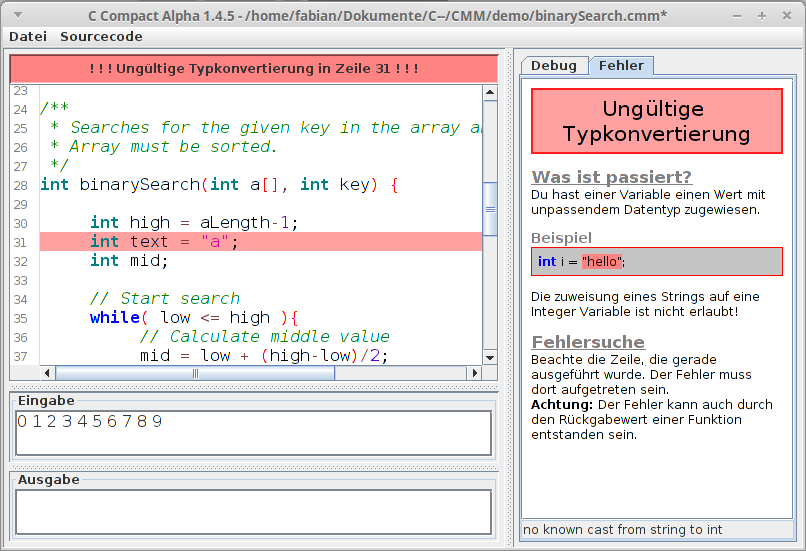
\includegraphics[width=0.8\textwidth]{./media/images/gui/debugger/gui-error-2.png}
\caption{Ein Fehler im Quelltext wird angezeigt}\label{fig:deb-error-gui}
\end{figure}

Diese Fehlerbeschreibungen werden im Ordner \textbf{error} in einem Unterordner mit dem jeweiligen Sprachkennzeichen --- zum Beispiel \textbf{de} für Deutsch --- als HTML-Dokumente gespeichert. Im Ordner \textbf{error} befinden sich außerdem die Dateien \textbf{table.xml} und \textbf{style.css}. In der Datei \textbf{table.xml} werden Fehlermeldungen einzelner Komponenten von C Compact mit der zugehörigen Beschreibungsdatei verknüpft. Dabei sind auch reguläre Ausdrücke erlaubt. Das Codebeispiel unten beinhaltet zuerst eine Zuweisung für mehrere ähnliche Fehlermeldungen und dann die Zuweisung eines bestimmten Fehlers zu einem Dokument. Der Pfad des Beschreibungsdokumentes wird unabhängig vom jeweiligen Sprachordner angegeben, sodass die Fehlermeldung in der eingestellten Sprache geladen werden kann.
\begin{lstlisting}[language=XML]
<error id="no known cast from ([\w./\s]+)">
	<file>cast.html</file>
</error>
<error id="variable assigment is not allowed in struct">
	<file>compiler/variable_decl/struct_var_assign.html</file>
</error>
\end{lstlisting}

Für unbekannte Fehlermeldungen ist die Datei \textbf{default.html} im jeweiligen Sprachordner vorhanden. Derzeit sind sind nur für die deutsche Übersetzung alle Fehlermeldungen ausgearbeitet. Auf Englisch sind also die meisten Fehlerbeschreibungen nicht verfügbar.

Die Datei \textbf{style.css} enthält die Formatierungsinformationen für die Fehlerdokumente


